\chapter{Sortiranje}

\index{sortiranje}

\key{Sortiranje}
je temeljni problem u dizajnu algoritama.
Mnogi efikasni algoritmi
koriste sortiranje kao potprogram,
jer je često lakše obraditi
podatke ako su elementi u sortiranom poretku.

Na primjer, zadatak ''sadrži li niz
dva jednaka elementa?'' lako je riješiti sortiranjem.
Ako niz sadrži dva jednaka elementa,
nakon sortiranja bit će jedan pored drugoga,
pa ih je lako pronaći.
Slično se može riješiti i zadatak ''koji je element
najčešći u nizu?''.

Postoji mnogo algoritama za sortiranje i oni su
ujedno dobri primjeri primjene
različitih tehnika dizajna algoritama.
Efikasni opći algoritmi za sortiranje
rade u $O(n \log n)$ vremenu,
a i mnogi algoritmi koji koriste sortiranje
kao potprogram također
imaju tu vremensku složenost.

\section{Teorija sortiranja}

Osnovni problem sortiranja glasi ovako:
\begin{framed}
\noindent
Zadan je niz koji sadrži $n$ elemenata,
a zadatak je sortirati elemente
u rastućem poretku.
\end{framed}
\noindent
Na primjer, niz
\begin{center}
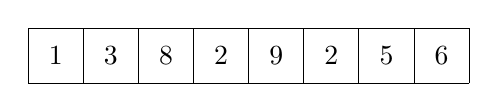
\begin{tikzpicture}[scale=0.7]
\draw (0,0) grid (8,1);
\node at (0.5,0.5) {$1$};
\node at (1.5,0.5) {$3$};
\node at (2.5,0.5) {$8$};
\node at (3.5,0.5) {$2$};
\node at (4.5,0.5) {$9$};
\node at (5.5,0.5) {$2$};
\node at (6.5,0.5) {$5$};
\node at (7.5,0.5) {$6$};
\end{tikzpicture}
\end{center}
nakon sortiranja izgledat će ovako:
\begin{center}
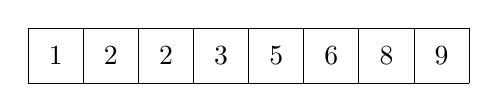
\begin{tikzpicture}[scale=0.7]
\draw (0,0) grid (8,1);
\node at (0.5,0.5) {$1$};
\node at (1.5,0.5) {$2$};
\node at (2.5,0.5) {$2$};
\node at (3.5,0.5) {$3$};
\node at (4.5,0.5) {$5$};
\node at (5.5,0.5) {$6$};
\node at (6.5,0.5) {$8$};
\node at (7.5,0.5) {$9$};
\end{tikzpicture}
\end{center}

\subsubsection{$O(n^2)$ algoritmi}

\index{bubble sort}

Jednostavni algoritmi za sortiranje niza
rade u $O(n^2)$ vremenu.
Takvi su algoritmi kratki i obično se
sastoje od dviju ugniježđenih petlji.
Poznati algoritam za sortiranje u $O(n^2)$ vremenu
je \key{bubble sort} u kojem elementi
''izranjaju'' u nizu prema svojim vrijednostima.

Bubble sort sastoji se od $n$ prolaza.
U svakom prolazu algoritam prolazi kroz
elemente niza.
Kad god pronađe dva uzastopna elementa
koja nisu u ispravnom poretku,
algoritam ih zamijeni.
Algoritam se može implementirati ovako:
\begin{lstlisting}
for (int i = 0; i < n; i++) {
    for (int j = 0; j < n-1; j++) {
        if (array[j] > array[j+1]) {
            swap(array[j],array[j+1]);
        }
    }
}
\end{lstlisting}

Nakon prvog prolaza algoritma
najveći element bit će na ispravnom mjestu,
a općenito, nakon $k$ prolaza $k$ najvećih
elemenata bit će na ispravnim mjestima.
Dakle, nakon $n$ prolaza cijeli niz
bit će sortiran.

Na primjer, u nizu

\begin{center}
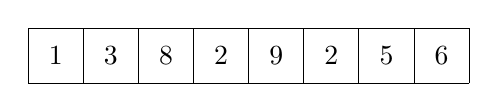
\begin{tikzpicture}[scale=0.7]
\draw (0,0) grid (8,1);

\node at (0.5,0.5) {$1$};
\node at (1.5,0.5) {$3$};
\node at (2.5,0.5) {$8$};
\node at (3.5,0.5) {$2$};
\node at (4.5,0.5) {$9$};
\node at (5.5,0.5) {$2$};
\node at (6.5,0.5) {$5$};
\node at (7.5,0.5) {$6$};
\end{tikzpicture}
\end{center}

\noindent
prvi prolaz algoritma bubble sort zamjenjuje elemente
ovako:

\begin{center}
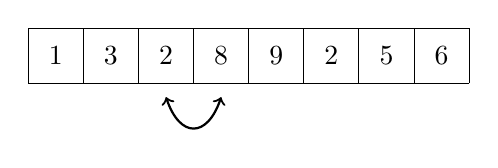
\begin{tikzpicture}[scale=0.7]
\draw (0,0) grid (8,1);
\node at (0.5,0.5) {$1$};
\node at (1.5,0.5) {$3$};
\node at (2.5,0.5) {$2$};
\node at (3.5,0.5) {$8$};
\node at (4.5,0.5) {$9$};
\node at (5.5,0.5) {$2$};
\node at (6.5,0.5) {$5$};
\node at (7.5,0.5) {$6$};

\draw[thick,<->] (3.5,-0.25) .. controls (3.25,-1.00) and (2.75,-1.00) .. (2.5,-0.25);
\end{tikzpicture}
\end{center}

\begin{center}
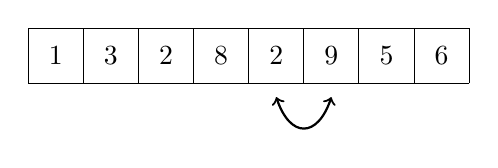
\begin{tikzpicture}[scale=0.7]
\draw (0,0) grid (8,1);
\node at (0.5,0.5) {$1$};
\node at (1.5,0.5) {$3$};
\node at (2.5,0.5) {$2$};
\node at (3.5,0.5) {$8$};
\node at (4.5,0.5) {$2$};
\node at (5.5,0.5) {$9$};
\node at (6.5,0.5) {$5$};
\node at (7.5,0.5) {$6$};

\draw[thick,<->] (5.5,-0.25) .. controls (5.25,-1.00) and (4.75,-1.00) .. (4.5,-0.25);
\end{tikzpicture}
\end{center}

\begin{center}
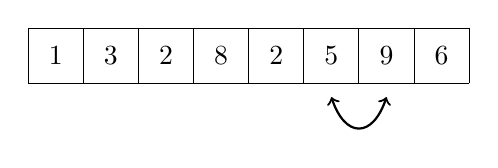
\begin{tikzpicture}[scale=0.7]
\draw (0,0) grid (8,1);
\node at (0.5,0.5) {$1$};
\node at (1.5,0.5) {$3$};
\node at (2.5,0.5) {$2$};
\node at (3.5,0.5) {$8$};
\node at (4.5,0.5) {$2$};
\node at (5.5,0.5) {$5$};
\node at (6.5,0.5) {$9$};
\node at (7.5,0.5) {$6$};

\draw[thick,<->] (6.5,-0.25) .. controls (6.25,-1.00) and (5.75,-1.00) .. (5.5,-0.25);
\end{tikzpicture}
\end{center}

\begin{center}
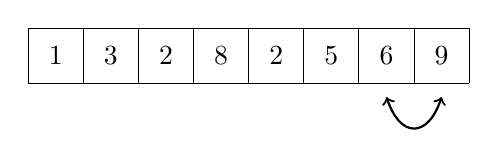
\begin{tikzpicture}[scale=0.7]
\draw (0,0) grid (8,1);
\node at (0.5,0.5) {$1$};
\node at (1.5,0.5) {$3$};
\node at (2.5,0.5) {$2$};
\node at (3.5,0.5) {$8$};
\node at (4.5,0.5) {$2$};
\node at (5.5,0.5) {$5$};
\node at (6.5,0.5) {$6$};
\node at (7.5,0.5) {$9$};

\draw[thick,<->] (7.5,-0.25) .. controls (7.25,-1.00) and (6.75,-1.00) .. (6.5,-0.25);
\end{tikzpicture}
\end{center}

\subsubsection{Inverzije}

\index{inverzija}

Bubble sort je primjer algoritma za
sortiranje koji uvijek zamjenjuje \emph{uzastopne}
elemente niza.
Pokazuje se da je vremenska složenost
takvog algoritma \emph{uvijek}
barem $O(n^2)$, jer je u najgorem slučaju
za sortiranje niza potrebno $O(n^2)$ zamjena.

Koristan pojam pri analizi algoritama
za sortiranje je \key{inverzija}:
par elemenata niza
$(\texttt{array}[a],\texttt{array}[b])$ takav da je
$a<b$ i $\texttt{array}[a]>\texttt{array}[b]$,
tj. elementi su u pogrešnom poretku.
Na primjer, niz
\begin{center}
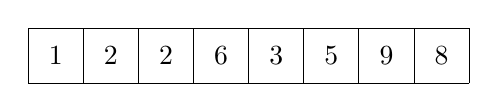
\begin{tikzpicture}[scale=0.7]
\draw (0,0) grid (8,1);
\node at (0.5,0.5) {$1$};
\node at (1.5,0.5) {$2$};
\node at (2.5,0.5) {$2$};
\node at (3.5,0.5) {$6$};
\node at (4.5,0.5) {$3$};
\node at (5.5,0.5) {$5$};
\node at (6.5,0.5) {$9$};
\node at (7.5,0.5) {$8$};
\end{tikzpicture}
\end{center}
ima tri inverzije: $(6,3)$, $(6,5)$ i $(9,8)$.
Broj inverzija pokazuje
koliko je posla potrebno za sortiranje niza.
Niz je potpuno sortiran kada
nema nijedne inverzije.
S druge strane, ako su elementi niza
u obrnutom poretku,
broj inverzija je najveći mogući:
\[1+2+\cdots+(n-1)=\frac{n(n-1)}{2} = O(n^2)\]

Zamjena para uzastopnih elemenata koji su
u pogrešnom poretku uklanja točno jednu inverziju
iz niza.
Stoga, ako algoritam za sortiranje može
zamjenjivati samo uzastopne elemente, svaka zamjena uklanja
najviše jednu inverziju, pa je vremenska složenost
algoritma barem $O(n^2)$.

\subsubsection{$O(n \log n)$ algoritmi}

\index{merge sort}

Niz je moguće efikasno sortirati
u $O(n \log n)$ vremenu pomoću algoritama
koji nisu ograničeni na zamjenu uzastopnih elemenata.
Jedan takav algoritam je \key{merge sort}\footnote{Prema \cite{knu983},
merge sort izmislio je J. von Neumann 1945. godine.},
koji se temelji na rekurziji.

Merge sort sortira podniz \texttt{array}$[a \ldots b]$ ovako:

\begin{enumerate}
\item Ako je $a=b$, ne radi ništa, jer je podniz već sortiran.
\item Izračunaj poziciju srednjeg elementa: $k=\lfloor (a+b)/2 \rfloor$.
\item Rekurzivno sortiraj podniz \texttt{array}$[a \ldots k]$.
\item Rekurzivno sortiraj podniz \texttt{array}$[k+1 \ldots b]$.
\item \emph{Spoji} sortirane podnizove \texttt{array}$[a \ldots k]$ i
\texttt{array}$[k+1 \ldots b]$
u sortirani podniz \texttt{array}$[a \ldots b]$.
\end{enumerate}

Merge sort je efikasan algoritam jer u
svakom koraku prepolovi veličinu podniza.
Rekurzija se sastoji od $O(\log n)$ razina,
a obrada svake razine traje $O(n)$ vremena.
Spajanje podnizova \texttt{array}$[a \ldots k]$ i \texttt{array}$[k+1 \ldots b]$
moguće je u linearnom vremenu jer su oni već sortirani.

Na primjer, razmotrimo sortiranje sljedećeg niza:
\begin{center}
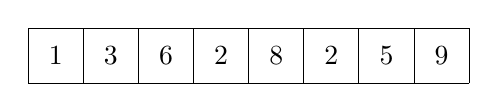
\begin{tikzpicture}[scale=0.7]
\draw (0,0) grid (8,1);
\node at (0.5,0.5) {$1$};
\node at (1.5,0.5) {$3$};
\node at (2.5,0.5) {$6$};
\node at (3.5,0.5) {$2$};
\node at (4.5,0.5) {$8$};
\node at (5.5,0.5) {$2$};
\node at (6.5,0.5) {$5$};
\node at (7.5,0.5) {$9$};
\end{tikzpicture}
\end{center}

Niz će biti podijeljen u dva podniza
ovako:
\begin{center}
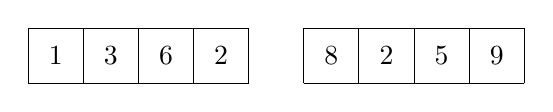
\begin{tikzpicture}[scale=0.7]
\draw (0,0) grid (4,1);
\draw (5,0) grid (9,1);

\node at (0.5,0.5) {$1$};
\node at (1.5,0.5) {$3$};
\node at (2.5,0.5) {$6$};
\node at (3.5,0.5) {$2$};

\node at (5.5,0.5) {$8$};
\node at (6.5,0.5) {$2$};
\node at (7.5,0.5) {$5$};
\node at (8.5,0.5) {$9$};
\end{tikzpicture}
\end{center}

Zatim će podnizovi biti rekurzivno sortirani
ovako:
\begin{center}
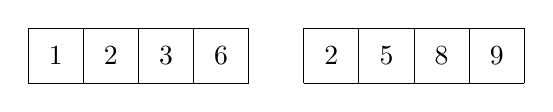
\begin{tikzpicture}[scale=0.7]
\draw (0,0) grid (4,1);
\draw (5,0) grid (9,1);

\node at (0.5,0.5) {$1$};
\node at (1.5,0.5) {$2$};
\node at (2.5,0.5) {$3$};
\node at (3.5,0.5) {$6$};

\node at (5.5,0.5) {$2$};
\node at (6.5,0.5) {$5$};
\node at (7.5,0.5) {$8$};
\node at (8.5,0.5) {$9$};
\end{tikzpicture}
\end{center}

Naposljetku, algoritam spaja sortirane
podnizove i stvara konačni sortirani niz:
\begin{center}
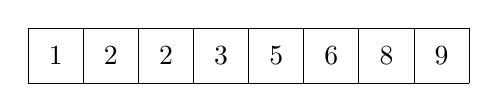
\begin{tikzpicture}[scale=0.7]
\draw (0,0) grid (8,1);
\node at (0.5,0.5) {$1$};
\node at (1.5,0.5) {$2$};
\node at (2.5,0.5) {$2$};
\node at (3.5,0.5) {$3$};
\node at (4.5,0.5) {$5$};
\node at (5.5,0.5) {$6$};
\node at (6.5,0.5) {$8$};
\node at (7.5,0.5) {$9$};
\end{tikzpicture}
\end{center}

\subsubsection{Donja ograda za sortiranje}

Je li moguće sortirati niz brže
nego u $O(n \log n)$ vremenu?
Pokazuje se da to \emph{nije} moguće
ako se ograničimo na algoritme za sortiranje
koji se temelje na uspoređivanju elemenata niza.

Donja ograda za vremensku složenost
može se dokazati promatranjem sortiranja
kao procesa u kojem svaka usporedba dvaju elemenata
daje više informacija o sadržaju niza.
Taj proces stvara sljedeće stablo:

\begin{center}
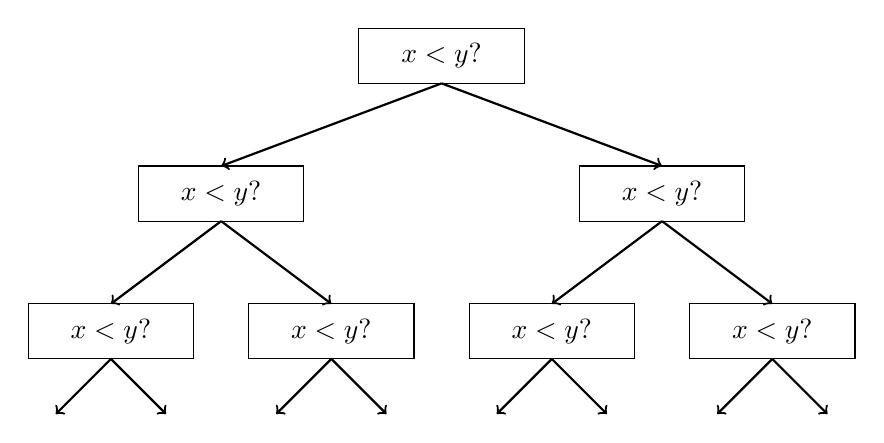
\begin{tikzpicture}[scale=0.7]
\draw (0,0) rectangle (3,1);
\node at (1.5,0.5) {$x < y?$};

\draw[thick,->] (1.5,0) -- (-2.5,-1.5);
\draw[thick,->] (1.5,0) -- (5.5,-1.5);

\draw (-4,-2.5) rectangle (-1,-1.5);
\draw (4,-2.5) rectangle (7,-1.5);
\node at (-2.5,-2) {$x < y?$};
\node at (5.5,-2) {$x < y?$};

\draw[thick,->] (-2.5,-2.5) -- (-4.5,-4);
\draw[thick,->] (-2.5,-2.5) -- (-0.5,-4);
\draw[thick,->] (5.5,-2.5) -- (3.5,-4);
\draw[thick,->] (5.5,-2.5) -- (7.5,-4);

\draw (-6,-5) rectangle (-3,-4);
\draw (-2,-5) rectangle (1,-4);
\draw (2,-5) rectangle (5,-4);
\draw (6,-5) rectangle (9,-4);
\node at (-4.5,-4.5) {$x < y?$};
\node at (-0.5,-4.5) {$x < y?$};
\node at (3.5,-4.5) {$x < y?$};
\node at (7.5,-4.5) {$x < y?$};

\draw[thick,->] (-4.5,-5) -- (-5.5,-6);
\draw[thick,->] (-4.5,-5) -- (-3.5,-6);
\draw[thick,->] (-0.5,-5) -- (0.5,-6);
\draw[thick,->] (-0.5,-5) -- (-1.5,-6);
\draw[thick,->] (3.5,-5) -- (2.5,-6);
\draw[thick,->] (3.5,-5) -- (4.5,-6);
\draw[thick,->] (7.5,-5) -- (6.5,-6);
\draw[thick,->] (7.5,-5) -- (8.5,-6);
\end{tikzpicture}
\end{center}

Ovdje ''$x<y?$'' znači da se uspoređuju
neki elementi $x$ i $y$.
Ako je $x<y$, proces se nastavlja ulijevo,
a inače udesno.
Rezultati procesa su mogući
načini sortiranja niza, njih ukupno $n!$.
Zbog toga visina stabla
mora biti barem
\[ \log_2(n!) = \log_2(1)+\log_2(2)+\cdots+\log_2(n).\]
Donju ogradu za tu sumu dobivamo
tako da odaberemo posljednjih $n/2$ elemenata i
promijenimo vrijednost svakog elementa u $\log_2(n/2)$.
To daje procjenu
\[ \log_2(n!) \ge (n/2) \cdot \log_2(n/2),\]
pa su visina stabla i najmanji
mogući broj koraka algoritma za
sortiranje u najgorem slučaju
barem $n \log n$.

\subsubsection{Counting sort}

\index{counting sort}

Donja ograda $n \log n$ ne odnosi se na
algoritme koji ne uspoređuju elemente niza,
nego koriste neku drugu informaciju.
Primjer takvog algoritma je
\key{counting sort} koji sortira niz u
$O(n)$ vremenu uz pretpostavku da je svaki element niza
cijeli broj između $0 \ldots c$ i da je $c=O(n)$.

Algoritam stvara \emph{pomoćni} niz
čiji su indeksi elementi izvornog niza.
Algoritam prolazi kroz izvorni niz
i računa koliko se puta svaki element
pojavljuje u nizu.
\newpage

Na primjer, niz
\begin{center}
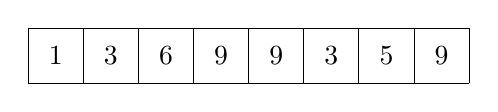
\begin{tikzpicture}[scale=0.7]
\draw (0,0) grid (8,1);
\node at (0.5,0.5) {$1$};
\node at (1.5,0.5) {$3$};
\node at (2.5,0.5) {$6$};
\node at (3.5,0.5) {$9$};
\node at (4.5,0.5) {$9$};
\node at (5.5,0.5) {$3$};
\node at (6.5,0.5) {$5$};
\node at (7.5,0.5) {$9$};
\end{tikzpicture}
\end{center}
odgovara sljedećem pomoćnom nizu:
\begin{center}
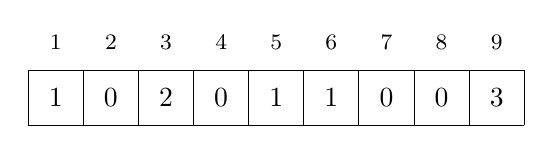
\begin{tikzpicture}[scale=0.7]
\draw (0,0) grid (9,1);
\node at (0.5,0.5) {$1$};
\node at (1.5,0.5) {$0$};
\node at (2.5,0.5) {$2$};
\node at (3.5,0.5) {$0$};
\node at (4.5,0.5) {$1$};
\node at (5.5,0.5) {$1$};
\node at (6.5,0.5) {$0$};
\node at (7.5,0.5) {$0$};
\node at (8.5,0.5) {$3$};

\footnotesize

\node at (0.5,1.5) {$1$};
\node at (1.5,1.5) {$2$};
\node at (2.5,1.5) {$3$};
\node at (3.5,1.5) {$4$};
\node at (4.5,1.5) {$5$};
\node at (5.5,1.5) {$6$};
\node at (6.5,1.5) {$7$};
\node at (7.5,1.5) {$8$};
\node at (8.5,1.5) {$9$};
\end{tikzpicture}
\end{center}

Na primjer, vrijednost na poziciji 3
u pomoćnom nizu je 2,
jer se element 3 pojavljuje 2 puta
u izvornom nizu.

Konstrukcija pomoćnog niza
traje $O(n)$ vremena. Nakon toga se sortirani niz
može stvoriti u $O(n)$ vremenu jer se
broj pojavljivanja svakog elementa može očitati
iz pomoćnog niza.
Dakle, ukupna vremenska složenost algoritma counting
sort je $O(n)$.

Counting sort je vrlo efikasan algoritam,
ali se može koristiti samo kada je konstanta $c$
dovoljno malena, tako da se elementi niza mogu
koristiti kao indeksi u pomoćnom nizu.

\section{Sortiranje u C++-u}

\index{sort@\texttt{sort}}

Gotovo nikad nije dobra ideja koristiti
vlastiti algoritam za sortiranje
na natjecanju, jer u programskim jezicima
postoje dobre gotove implementacije.
Na primjer, standardna biblioteka C++-a sadrži
funkciju \texttt{sort} koja se lako može koristiti za
sortiranje nizova i drugih struktura podataka.

Korištenje funkcije iz biblioteke ima mnogo prednosti.
Prvo, štedi vrijeme jer nema potrebe
implementirati funkciju.
Drugo, implementacija iz biblioteke je
sigurno ispravna i efikasna: nije vjerojatno
da bi vlastita funkcija za sortiranje bila bolja.

U ovom poglavlju vidjet ćemo kako se koristi
C++ funkcija \texttt{sort}.
Sljedeći kod sortira
vektor u rastućem poretku:
\begin{lstlisting}
vector<int> v = {4,2,5,3,5,8,3};
sort(v.begin(),v.end());
\end{lstlisting}
Nakon sortiranja sadržaj
vektora bit će
$[2,3,3,4,5,5,8]$.
Zadani poredak sortiranja je rastući,
ali je obrnuti poredak moguće dobiti ovako:
\begin{lstlisting}
sort(v.rbegin(),v.rend());
\end{lstlisting}
Obični niz može se sortirati ovako:
\begin{lstlisting}
int n = 7; // array size
int a[] = {4,2,5,3,5,8,3};
sort(a,a+n);
\end{lstlisting}
\newpage
Sljedeći kod sortira znakovni niz \texttt{s}:
\begin{lstlisting}
string s = "monkey";
sort(s.begin(), s.end());
\end{lstlisting}
Sortiranje znakovnog niza znači da se sortiraju
znakovi tog niza.
Na primjer, znakovni niz ''monkey'' postaje ''ekmnoy''.

\subsubsection{Operatori usporedbe}

\index{operator usporedbe}

Funkcija \texttt{sort} zahtijeva da je
za tip podataka elemenata koji se sortiraju
definiran \key{operator usporedbe}.
Pri sortiranju taj se operator koristi
kad god je potrebno utvrditi poredak dvaju elemenata.

Većina tipova podataka u C++-u ima ugrađeni operator usporedbe,
pa se elementi tih tipova mogu automatski sortirati.
Na primjer, brojevi se sortiraju prema svojim vrijednostima,
a znakovni nizovi abecednim redom.

\index{pair@\texttt{pair}}

Parovi (\texttt{pair}) sortiraju se prvenstveno prema svojim
prvim elementima (\texttt{first}).
Međutim, ako su prvi elementi dvaju parova jednaki,
sortiraju se prema svojim drugim elementima (\texttt{second}):
\begin{lstlisting}
vector<pair<int,int>> v;
v.push_back({1,5});
v.push_back({2,3});
v.push_back({1,2});
sort(v.begin(), v.end());
\end{lstlisting}
Nakon toga poredak parova je
$(1,2)$, $(1,5)$ i $(2,3)$.

\index{tuple@\texttt{tuple}}

Na sličan način, n-torke (\texttt{tuple})
sortiraju se prvenstveno prema prvom elementu,
zatim prema drugom elementu itd.\footnote{Imajte na umu da se u nekim starijim prevoditeljima (compiler)
za stvaranje n-torke mora koristiti funkcija \texttt{make\_tuple} umjesto
vitičastih zagrada (na primjer, \texttt{make\_tuple(2,1,4)} umjesto \texttt{\{2,1,4\}}).}:
\begin{lstlisting}
vector<tuple<int,int,int>> v;
v.push_back({2,1,4});
v.push_back({1,5,3});
v.push_back({2,1,3});
sort(v.begin(), v.end());
\end{lstlisting}
Nakon toga poredak n-torki je
$(1,5,3)$, $(2,1,3)$ i $(2,1,4)$.

\subsubsection{Korisnički definirane strukture}

Korisnički definirane strukture nemaju automatski
operator usporedbe.
Operator treba definirati unutar
strukture kao funkciju
\texttt{operator<},
čiji je parametar drugi element istog tipa.
Operator treba vratiti \texttt{true}
ako je element manji od parametra,
a \texttt{false} inače.

Na primjer, sljedeća struktura \texttt{P}
sadrži x i y koordinate točke.
Operator usporedbe definiran je tako da se
točke sortiraju prvenstveno po x koordinati,
a zatim po y koordinati.

\begin{lstlisting}
struct P {
    int x, y;
    bool operator<(const P &p) {
        if (x != p.x) return x < p.x;
        else return y < p.y;
    }
};
\end{lstlisting}

\subsubsection{Funkcije usporedbe}

\index{funkcija usporedbe}

Funkciji \texttt{sort} moguće je zadati i vanjsku
\key{funkciju usporedbe}
kao povratnu (callback) funkciju.
Na primjer, sljedeća funkcija usporedbe \texttt{comp}
sortira znakovne nizove prvenstveno po duljini, a zatim
abecednim redom:

\begin{lstlisting}
bool comp(string a, string b) {
    if (a.size() != b.size()) return a.size() < b.size();
    return a < b;
}
\end{lstlisting}
Sada se vektor znakovnih nizova može sortirati ovako:
\begin{lstlisting}
sort(v.begin(), v.end(), comp);
\end{lstlisting}

\section{Binarno traženje}

\index{binarno traženje}

Općenit način traženja elementa
u nizu je korištenje \texttt{for} petlje
koja prolazi kroz elemente niza.
Na primjer, sljedeći kod traži
element $x$ u nizu:

\begin{lstlisting}
for (int i = 0; i < n; i++) {
    if (array[i] == x) {
        // x found at index i
    }
}
\end{lstlisting}

Vremenska složenost ovog pristupa je $O(n)$,
jer je u najgorem slučaju potrebno provjeriti
sve elemente niza.
Ako je poredak elemenata proizvoljan,
to je ujedno i najbolji mogući pristup, jer
nema dodatne informacije o tome gdje
u nizu trebamo tražiti element $x$.

Međutim, ako je niz \emph{sortiran},
situacija je drugačija.
U tom je slučaju moguće provesti
traženje mnogo brže, jer poredak
elemenata u nizu usmjerava traženje.
Sljedeći algoritam \key{binarnog traženja}
efikasno traži element u sortiranom nizu
u $O(\log n)$ vremenu.

\subsubsection{Metoda 1}

Uobičajen način implementacije binarnog traženja
nalikuje traženju riječi u rječniku.
Traženje održava aktivno područje u nizu,
koje na početku sadrži sve elemente niza.
Zatim se izvodi niz koraka,
od kojih svaki prepolovi veličinu tog područja.

U svakom koraku traženje provjerava srednji element
aktivnog područja.
Ako je srednji element traženi element,
traženje završava.
Inače se traženje rekurzivno nastavlja
u lijevoj ili desnoj polovici područja,
ovisno o vrijednosti srednjeg elementa.

Gornja se ideja može implementirati ovako:
\begin{lstlisting}
int a = 0, b = n-1;
while (a <= b) {
    int k = (a+b)/2;
    if (array[k] == x) {
        // x found at index k
    }
    if (array[k] > x) b = k-1;
    else a = k+1;
}
\end{lstlisting}

U ovoj implementaciji aktivno područje je $a \ldots b$,
a na početku je područje $0 \ldots n-1$.
Algoritam u svakom koraku prepolovi veličinu područja,
pa je vremenska složenost $O(\log n)$.

\subsubsection{Metoda 2}

Alternativna metoda implementacije binarnog traženja
temelji se na efikasnom načinu prolaska kroz
elemente niza.
Ideja je raditi skokove i usporavati
kada se približimo traženom elementu.

Traženje prolazi kroz niz slijeva
nadesno, a početna duljina skoka je $n/2$.
U svakom će se koraku duljina skoka prepoloviti:
najprije $n/4$, zatim $n/8$, $n/16$ itd., sve dok
naposljetku duljina ne postane 1.
Nakon skokova ili je traženi element
pronađen ili znamo da se ne pojavljuje u nizu.

Sljedeći kod implementira gornju ideju:
\begin{lstlisting}
int k = 0;
for (int b = n/2; b >= 1; b /= 2) {
    while (k+b < n && array[k+b] <= x) k += b;
}
if (array[k] == x) {
    // x found at index k
}
\end{lstlisting}

Tijekom traženja varijabla $b$
sadrži trenutnu duljinu skoka.
Vremenska složenost algoritma je $O(\log n)$,
jer se kod u \texttt{while} petlji
izvodi najviše dvaput za svaku duljinu skoka.

\subsubsection{C++ funkcije}

Standardna biblioteka C++-a sadrži sljedeće funkcije
koje se temelje na binarnom traženju i rade u logaritamskom vremenu:

\begin{itemize}
\item \texttt{lower\_bound} vraća pokazivač na
prvi element niza čija je vrijednost barem $x$.
\item \texttt{upper\_bound} vraća pokazivač na
prvi element niza čija je vrijednost veća od $x$.
\item \texttt{equal\_range} vraća oba gornja pokazivača.
\end{itemize}

Funkcije pretpostavljaju da je niz sortiran.
Ako takvog elementa nema, pokazivač pokazuje na
element iza posljednjeg elementa niza.
Na primjer, sljedeći kod utvrđuje sadrži li
niz element s vrijednošću $x$:

\begin{lstlisting}
auto k = lower_bound(array,array+n,x)-array;
if (k < n && array[k] == x) {
    // x found at index k
}
\end{lstlisting}

Zatim, sljedeći kod broji koliko elemenata
ima vrijednost $x$:

\begin{lstlisting}
auto a = lower_bound(array, array+n, x);
auto b = upper_bound(array, array+n, x);
cout << b-a << "\n";
\end{lstlisting}

Uz \texttt{equal\_range} kod postaje kraći:

\begin{lstlisting}
auto r = equal_range(array, array+n, x);
cout << r.second-r.first << "\n";
\end{lstlisting}

\subsubsection{Traženje najmanjeg rješenja}

Važna primjena binarnog traženja je
pronalaženje pozicije na kojoj se mijenja vrijednost \emph{funkcije}.
Pretpostavimo da želimo pronaći najmanju vrijednost $k$
koja je valjano rješenje zadatka.
Zadana nam je funkcija $\texttt{ok}(x)$
koja vraća \texttt{true} ako je $x$ valjano rješenje,
a \texttt{false} inače.
Osim toga, znamo da je $\texttt{ok}(x)$ jednako \texttt{false}
kada je $x<k$, a \texttt{true} kada je $x \ge k$.
Situacija izgleda ovako:

\begin{center}
\begin{tabular}{r|rrrrrrrr}
$x$ & 0 & 1 & $\cdots$ & $k-1$ & $k$ & $k+1$ & $\cdots$ \\
\hline
$\texttt{ok}(x)$ & \texttt{false} & \texttt{false}
& $\cdots$ & \texttt{false} & \texttt{true} & \texttt{true} & $\cdots$ \\
\end{tabular}
\end{center}

\noindent
Sada se vrijednost $k$ može pronaći binarnim traženjem:

\begin{lstlisting}
int x = -1;
for (int b = z; b >= 1; b /= 2) {
    while (!ok(x+b)) x += b;
}
int k = x+1;
\end{lstlisting}

Traženje pronalazi najveću vrijednost $x$ za koju
je $\texttt{ok}(x)$ jednako \texttt{false}.
Stoga je sljedeća vrijednost $k=x+1$
najmanja moguća vrijednost za koju
je $\texttt{ok}(k)$ jednako \texttt{true}.
Početna duljina skoka $z$ mora biti
dovoljno velika, na primjer neka vrijednost
za koju unaprijed znamo da je $\texttt{ok}(z)$ jednako \texttt{true}.

Algoritam poziva funkciju \texttt{ok}
$O(\log z)$ puta, pa ukupna vremenska složenost
ovisi o funkciji \texttt{ok}.
Na primjer, ako funkcija radi u $O(n)$ vremenu,
ukupna vremenska složenost je $O(n \log z)$.

\subsubsection{Traženje najveće vrijednosti}

Binarno traženje može se koristiti i za pronalaženje
najveće vrijednosti funkcije koja
najprije raste, a zatim pada.
Naš je zadatak pronaći poziciju $k$ takvu da vrijedi

\begin{itemize}
\item
$f(x)<f(x+1)$ kada je $x<k$, i
\item
$f(x)>f(x+1)$ kada je $x \ge k$.
\end{itemize}

Ideja je binarnim traženjem
pronaći najveću vrijednost $x$
za koju je $f(x)<f(x+1)$.
Iz toga slijedi $k=x+1$
jer je $f(x+1)>f(x+2)$.
Sljedeći kod implementira to traženje: 

\begin{lstlisting}
int x = -1;
for (int b = z; b >= 1; b /= 2) {
    while (f(x+b) < f(x+b+1)) x += b;
}
int k = x+1;
\end{lstlisting}

Primijetite da, za razliku od običnog binarnog traženja,
ovdje nije dopušteno da uzastopne vrijednosti
funkcije budu jednake.
U tom slučaju ne bi bilo moguće znati
kako nastaviti traženje.
